\begin{minipage}{0.65\linewidth}
    On fixe un solide $\mathrm{(S)}$ de masse $m$ à un ressort $R$, à spires non
    jointives de masse négligeable et de raideur $K$, on obtient un oscillateur
    horizontal qui oscille sans frottements sur un rail horizontal.
    
    On étudie le mouvement du centre d'inertie $G$ du solide $\mathrm{(S)}$ dans
    un repère $(O,\ex)$ lié à la Terre supposé galiléen
    (Fig.~\ref{fig:solide_ressort}). À l'équilibre $x_{G}=x_{0}=0$.
\end{minipage}
\hfill
\begin{minipage}{0.34\linewidth}
    \begin{figure}[H]
        \centering
        \input{figures/solide_ressort}
        \caption{}
        \label{fig:solide_ressort}
    \end{figure}
\end{minipage}

On écarte $\mathrm{(S)}$ de sa position d'équilibre d'une distance $X_{m}$ et on
l'abandonne sans vitesse initiale à l'instant $t_{0}=0$, le solide
$\mathrm{(S)}$ est alors animé d'un mouvement de translation rectiligne
sinusoïdal d'équation
${x_{G}(t)=X_{m}\cdot\cos\left(\frac{2\pi}{T_{0}}t+\varphi\right)}$.

\begin{minipage}[t][][t]{0.60\linewidth}
La courbe de la Fig.~\ref{fig:tdb_2bac_svt_national_2025_normale_phys_ex3_3}
donne le diagramme des espaces $x_{G}(t)$ obtenu.

\textbf{Données~:} $m=\qty{200}{\g}$
\begin{enumerate}
    \item Déterminer graphiquement la valeur de la période propre $T_{0}$ de
          l'oscillateur et celle de l'amplitude $X_{m}$ des oscillations.
    \item Écrire l'expression numérique de l'équation horaire du mouvement de
          $G$.
    \item On choisit l'état où le ressort n'est pas déformé comme état de
          référence de l'énergie potentielle élastique $E_{pe}$ et le plan
          horizontal contenant $G$ comme état de référence de l'énergie
          potentielle de pesanteur $E_{pp}$.

          La courbe de la
          Fig.~\ref{fig:tdb_2bac_svt_national_2025_normale_phys_ex3_4} donne le
          diagramme de l'énergie potentielle élastique $E_{pe}$ de l'oscillateur
          (solide - ressort).
          \begin{enumerate}
              \item Déterminer graphiquement la valeur maximale $E_{pe,\max}$ de
                    l'énergie potentielle élastique.
              \item Déduire la valeur de la raideur $K$ du ressort.
              \item Déterminer la valeur de l'énergie cinétique du solide
                    lorsque $G$ passe par la position d'élongation
                    ${x_{G}=\qty{0.02}{\m}}$.
          \end{enumerate}
\end{enumerate}
\end{minipage}
\hfill
\begin{minipage}[t][][t]{0.38\linewidth}
    \vspace{-5mm}
    \begin{figure}[H]
        \centering
        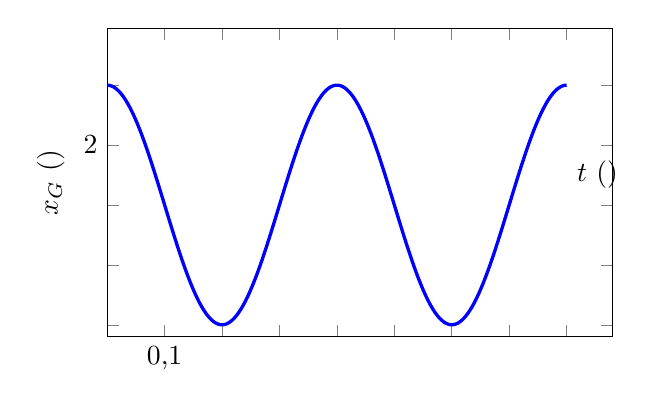
\begin{tikzpicture}
            \def\Xm{4}
            \def\T{0.4}
            \pgfmathpi\let\pi=\pgfmathresult
            \begin{axis}[
                    xmin=0,xmax=2.2*\T,
                    ymin=-4.4,ymax=5.9,
                    width=8cm,height=5.5cm,
                    trig format plots=rad,
                    xtick distance=0.1, ytick distance=2,
                    xticklabels={,,{0,1}}, yticklabels={,,,,{2}},
                    xlabel=$t~(\unit{\second})$, ylabel=$x_{G}~(\unit{\cm})$,
                    every axis x label/.append style={
                        at={(1.03,0.45)},anchor=south east,
                    },
                    minor tick num=0,
                ]
                \addplot[domain=0:2*\T,samples=200,very thick,blue]
                    {\Xm*cos(2*pi/\T*x)};
            \end{axis}
        \end{tikzpicture}
        \caption{}
        \label{fig:tdb_2bac_svt_national_2025_normale_phys_ex3_3}
    \end{figure}
    \begin{figure}[H]
        \centering
        \begin{tikzpicture}
            \def\K{50}
            \def\Xm{0.04}
            \begin{axis}[
                    xmin=-0.045,xmax=0.045,
                    ymin=0,ymax=55,
                    width=8cm,height=5.5cm,
                    xlabel=$x~(\unit{\meter})$,
                    ylabel=$E_{pe}~(\unit{\mJ})$,
                    every axis y label/.append style={
                        at={(0.55,0.95)},anchor=west,
                    },
                    scaled ticks=false,
                    xtick distance=0.01, ytick distance=10,
                    xticklabels={,,,,,,{0,01}}, yticklabels={,,{10}},
                    minor tick num=0,
                ]
                \addplot[domain=-\Xm:\Xm,samples=200,
                    very thick,blue] {0.5*\K*x^2*1e3}
                    coordinate[pos=0](A) coordinate[pos=1](B);
            \end{axis}
            \foreach \n/\a in {A/200,B/-20}{%
            \draw[very thick] ([yshift=-5mm]\n) -- ([yshift=5mm]\n);
            \foreach \f in {0.02,0.14,...,1}
                \draw[thick]
                    ($([yshift=-5mm]\n)!\f!([yshift=5mm]\n)$) -- ++(\a:.2);
            }
        \end{tikzpicture}
        \caption{}
        \label{fig:tdb_2bac_svt_national_2025_normale_phys_ex3_4}
    \end{figure}
\end{minipage}




